\chapter{INTRODUCTION}
\label{sec:Introduction}

The Standard Model of Particle Physics (SM) is a quantum field theory (QFT) describing strong and electroweak (EW) interactions.
It was formulated in his current form in the mid-70s and has been an extremely successful and predictive theory since then.
Almost all known phenomena from 1 eV up to almost 200 GeV are well described by the SM and experiments at the Large Hadron
Collider (LHC) are now probing the SM up to the TeV scale.
Finally, in 2013 we were able to observe the Higgs boson, one of the fundamental building blocks of the theory,
giving a solid theoretical basis to the theory. However, experimentally well established effects, like neutrino
oscillations and the presence of dark matter, are outside the reach of the SM. Furthermore, the model does not include
the description of gravity. Therefore this motivates the search for New Physics (NP).

\begin{table}[h!]
\label{interactions}
\begin{tabular}{|c|c|c|c|c|}
Interaction	& Mediator	& Rel. strength	& Range	(m)	& Mediator mass (GeV/c${}^2$) \\
\hline
Strong		& $g$		& 1			& $\infty$		& 0		\\
EM		& $\gamma$	& $10^{-3}$		& $\infty$ 		& 0		\\
weak		& $Z$, $W^\pm$	& $10^{-16}$		& $10^{-18}$	& $W^\pm = 80.399$ \\
		&		&			&		& $Z_0 = 91.188$	\\
Gravity		& $g^0$ (graviton?) & $10^{-41}$	& $\infty$		& 0		\\
\end{tabular}
\caption{Fundamental forces of nature together with their gauge bosons, relative strengths and range.
Gravity is not included in the SM and the graviton is hypothetical at the current time.}
\end{table}

The SM is based on the symmetry groups of strong ($SU(3)_C$) and electroweak interactions ($SU(2)_L \times U(1)_Y$).
The subscripts C, L,and Y stand for colour, charge, left-handed fields, and hyper-charge. The Lagrangian describing the
SM has been then developed on invariance under the unitary product group $SU(3) \times SU(2) \times U(1)$, which reflects
conservation laws such as the conservation of electric and strong charge.
The parameters of the model were then experimentally measured.

Particles included in the SM can be grouped under a few categories depending on their properties and ability to interact with
each other. First of all we can distinguish between fermions (half-integer spin particles) and bosons (integer spin particles).
Fermions constitute the basic building blocks of matter, while bosons are the the mediators of the interaction between them.
Since in the SM the concept of bosonic mediators of interactions arises because of gauge symmetry\cite{Glashow:1961tr},
they are called ``gauge bosons". The list of the known interactions with their force carrier and properties is reported
in Table \ref{interactions}. The matter of which we are made is mainly composed of electrons and protons, which have spin 1/2;
protons are then composed of $u$ and $d$ quark, which again have spin 1/2. Among fermions one can then consider two smaller
groups: quarks and leptons. Quarks carry colour charge and therefore can interact through the, so called, strong interaction,
while leptons, which do not carry colour charge, are insensitive to it.
For each particle exists a corresponding anti-particle with opposite quantum numbers.
Finally fermions seem to be divided in three families having similar properties but different mass.
This last structure embedded in the SM is also calle flavour structure and it will be the main tool
used in this thesis, a more detailed description of it is given in the next sections.
A schematic view of the fundamental particles in the SM is shown in Fig.~\ref{fig:SMparticles}.

\begin{figure}[h]
\centering
\includegraphics[width=0.6\textwidth]{Introduction/figs/StandardModel3.png}
\caption{Diagram of SM particles with their properties \cite{SMimage}.}
\label{fig:SMparticles}
\end{figure}






\section{Electromagnetic and weak interactions}

The Electromagnetic (EM) force is responsible for binding electrons and nuclei together in atoms.
Its force carrier, the photon, is the gauge boson of the EM force. In the SM the photon must be massless,
which also sets the range of the EM force to infinity, since it is proportional to the inverse of the mediator mass.
In fact Heisenberg's Uncertainty Principle tells us that $\Delta E \Delta t > \hbar$, namely virtual particles
of energy $\Delta E$ are allowed to exist for time intervals inferior to $\Delta t$. Then, since they can move
at maximum at the velocity of light this also sets a relation between the length of time and space in which a virtual
photons can exist. The EM force has an infinite range as virtual photons can be very close to the mass shell, which results
in a very long lifetime.

The weak interaction is responsible for the $\beta$ decay of nuclei and all known fermions interact through the weak
interaction. In the Standard Model of particle physics this interaction is caused by the emission or absorption of $W^\pm$
and $Z$ bosons. These are much heavier than protons or neutrons (see Table \ref{interactions}) and this yields that the weak
force has a very short range. Using Heisenberg's Principle together with Einstein's formula $\Delta E = m c^2$, which relates
mass and energy, and knowing that the maximum space that a particle can cover in a time $\Delta t$ is $r = c \Delta t$,
qualitatively $r \sim \hbar / mc$. In this picture the carriers of the weak force can travel $r \sim 2 \cdot 10^{-3}$ fm.
The weak interaction is also the only one that violates parity-symmetry, which states that interactions are invariant under
a reflection of all coordinates. This symmetry breaking arises from the fact that only left-handed fermions interact through
the weak interaction. The first experiment showing this was made by Wu in 1957 \cite{Wu:1957my}. Similarly, the weak interaction
is the only one that also breaks the CP symmetry, which combines parity transformations and ``charge conjugation".
This is interesting also because all interactions are invariant under CPT transformations, which combines CP transformations
and time reversal, hence, breaking CP the weak interaction is also not invariant under time reversal.

In 1968 Salam, Glasow and Weinberg unified the weak and electromagnetic force in a single theory called electroweak (EW),
having a single coupling constant\cite{PDG2012}. The EW interactions are divided into charged currents (CC) and neutral
currents (NC). In the first group, quarks and leptons interact with the $W^\pm$ bosons, as in the decays
$\mu^+(\mu^-) \rightarrow e^+ \nu_e \bar{\nu_\mu} (e^- \bar{\nu_e} \nu_\mu)$ and $n \rightarrow p e^- \bar{\nu_e} (\bar{p} e^+ \nu_e)$.
The study of these processes confirmed that only the left-handed (right-handed) component of fermions (anti-fermions)
takes part in weak processes. The CC interaction have a peculiarity: they are the only interactions in the SM that violate
flavour conservation at tree level (see next section), while any other interaction not conserving flavour has to happen through
loops. The second group of EW interactions, NC, corresponds to interactions of the photon and $Z$ boson with a fermion
and its anti-fermion.

%The EM theory results from requiring the fermion Lagrangian to be invariant under local gauge transformations.
%The electron and positron free fermionic fields are defined as $\psi(x)$ and $\bar{\psi(x)}$, where x is a relativistic four vector.
%A local gauge transformation can always be written as:
%
%\begin{align}
%\psi(x) \rightarrow \psi(x') = e^i{\alpha(x)}\psi(x)
%\end{align}
%
%where $\alpha(x)$ can be any function of space and/or time. The free fermion Lagrangian, given by
%
%\begin{equation}
%\mathcal{L} = -i \bar{\psi(x)} \gamma^mu \partial_\mu \psi(x) - m\bar{\psi(x)} \psi
%\end{equation}
%
%is not invariant under such transformations. Greek indices denote space-time directions and imply summation and $\gamma^i$ are the Dirac matrices. If we apply the local gauge transformation and we subtract the initial Lagrangian we get a remaining term
%
%\begin{equation}
%\Delta \mathcal{L} = \mathcal{L}' - \mathcal{L} = -i \bar{\psi}  \gamma^mu \psi \partial_\mu \alpha(x)
%\end{equation}
%
%In order to make the Lagrangian invariant we can introduce a vector field $A$, which transforms as described by Eq. \ref{gauge invariance},  to %compensate for the remaining term: this is the photon field.
%
%\begin{equation}
%\label{gauge invariance}
%A'_\mu = A_\mu -\frac{1}{e}\partial_\mu \alpha(x)
%\end{equation}
%
%Redefining then the field derivative $D_\mu = \partial_\mu - ieA_\mu$, we obtain the invariant Lagrangian:
%
%\begin{equation}
%\mathcal{L} = -i \bar{\psi(x)} \gamma^mu D_\mu \psi(x)  - m\bar{\psi(x)} \psi = -i \bar{\psi(x)} (\gamma^mu \partial_\mu  - m)\psi(x) + e\bar{\psi}  \gamma^mu \psi A_\mu
%\end{equation}





\subsection{Flavour and the CKM matrix}

``Flavour" in particle physics refers to the quark/lepton composition of a particle. The introduction of flavour quantum numbers
was motivated in order to explain why some decays, although kinematically allowed, have never been observed. All leptons have a
quantum number $L_l = 1$ (where $l = e,\mu,\tau$), which is conserved by all interactions. For example decays
like $\mu^- \rightarrow e^- \gamma $, which is kinematically possible, have never been observed, since the lepton number
in the initial and final state are different, while decays conserving the lepton number as
$\mu^- \rightarrow e^- \nu_\mu \bar{\nu_e}$ have been observed.

In the non leptonic sector particles carry flavour numbers described as follow:

 \begin{itemize}
 \item \emph{Isospin}: $I_3 = 1/2$ for the up quark and value $I_3 = -1/2$ for the down quark;
 \item \emph{Strangeness}: $S = -(n_s - \bar{n}_s)$, where $n_s$ is the number of strange quarks and $\bar{n}_s$ is the number of anti-strange quarks;
 \item \emph{charmness, bottomness, topness}: in analogy to strangeness
 they are respectively defined as $C = -(n_c - \bar{n}_c)$, $B = -(n_b - \bar{n}_b)$, $T = -(n_t - \bar{n}_t)$.
 \end{itemize}

As mentioned before in the SM the only interaction violating flavour conservation is the weak interaction,
when mediated by $W^\pm$ bosons.

Measuring branching fractions of weak decays like $\pi \rightarrow \mu \nu_\mu$ and $K \rightarrow \mu \nu_\mu$, 
suggested the existence of more than one coupling constant. Cabibbo\cite{PDG2012}, in order to preserve the universality
of weak interactions, suggested that the difference in branching fraction could arise from the fact that
the doublets participating in the weak interactions are a mixture of the flavour eigenstates. He therefore introduced
the Cabibbo angle $\theta_c$ considering that eigenstates participating to the weak interaction are rotated with respect
of the flavour eigenstates.

\begin{equation}
\left( \begin{array}{c}
d_W \\ s_W
\end{array} \right) =
\left( \begin{array}{cc}
\cos \theta_c  & \sin \theta_c\\
-\sin \theta_c & \cos \theta_c
\end{array} \right)
\left( \begin{array}{c}
d \\ s
\end{array} \right) = 
\left( \begin{array}{c}
\cos\theta_c \cdot d + \sin \theta_c \cdot s \\
\cos \theta_c \cdot s - \sin \theta_c \cdot d
\end{array} \right)
\end{equation}

Considering a 6 quark system one angle is not enough to describe a rotation but the mixing system can be generalised
using a $3 \times 3$ unitary matrix, this is called CKM matrix, from the names of Cabibbo, Kobayashi and Maskawa.
The unitarity of the matrix is required in order to conserve the total probability. Theoretically, a $N \times N$ complex
matrix is dependent on $2 \cdot N^2$ real parameters. Then, requiring unitarity ($AA^\dagger = A(A^*)^T = I$),
the number of independent parameters left is $(N - 1)^2$. A $3 \times 3$ depends then on 4 real parameters, which
can be divided in 3 real constants and one imaginary phase. The imaginary phase generates the CP-violation which was
observed in weak interactions. In Eq. \ref{CKM} is reported a parametrisation of the CKM matrix together with the most
recent measured values\cite{PDG2012}. In this parametrisation $\rho$, $A$, and $\lambda$ are the real constants and $\eta$
the imaginary phase; in Eq. \ref{params} are reported their relations with the 3 mixing angles.

\begin{multline}
\label{CKM}
V_{CKM} = \left( \begin{array}{ccc}
1 - \lambda^2/2 & \lambda  & A \lambda^3(\rho -\i\eta) \\
-\lambda & 1 - \lambda^2/2 & A\lambda^2 \\
A \lambda^3(1 - \rho -\i\eta) & A\lambda^2 & 1 
\end{array} \right) + O(\lambda^3)= \\
= \left( \begin{array}{ccc}
0.97427 \pm 0.00015 & 0.22534 \pm 0.00065 & 0.00351^{+0.00015}_{-0.0014} \\
 0.22520 \pm 0.00065 & 0.97344 \pm 0.00016 & 0.00412^{+0.0011}_{-0.0005} \\
 0.00867^{+0.00029}_{-0.00031} & 0.0404^{+0.0011}_{-0.0005} & 0.999146^{+0.000021}_{-0.000046} \\
\end{array} \right)
\end{multline}

\begin{align}
\label{params}
\lambda & = \sin(\theta_{12}) = \sin(\theta_c) \\
A\lambda^2 & = \sin(\theta_{23}) \\
A\lambda^3(\rho - i\eta) & = \sin(\theta_{13})e^{i\delta}
\end{align}

It is interesting to note that the CKM matrix seems to be hierarchical, namely elements on the diagonal are approximately
1 and then get smaller and smaller going farther from the diagonal.
An other feature to note is that, due to the unitarity of the matrix, the transformation have no effect on neutral interaction.
As a result flavour-changing neutral currents are forbidden at tree level (in absence of closed loops) in the SM.

The CKM matrix to preserve probability has to be unitary and this imposes constraints to its terms for the form:
\begin{equation}
\sum_i |V_{ik}|^2 = 1 \text{ and } \sum_k V_{ik} V^{*}_{jk} = 0.
\end{equation}
This is a contraint of 3 complex numbers that can be viewed as the sides of a triangle called
the ``unitarity triangle". The precise measurement of the parameters of the unitarity triangle
is a powerful stability test of the standard model and sets a solid base for new physics
searches in the favour sector.

In Fig.~\ref{fig:unitarity_triangle} is shown a representation
of the unitarity triangle together with a plot summarising the most up to date contraints
the the angles from measurements. One of the main goals of the LHCb experiment is to precisely
measure the angle $\gamma$, which is currently the least constrained from measurements.
 
 \begin{figure}[h!]
\label{fig:unitarity_triangle}
\centering 
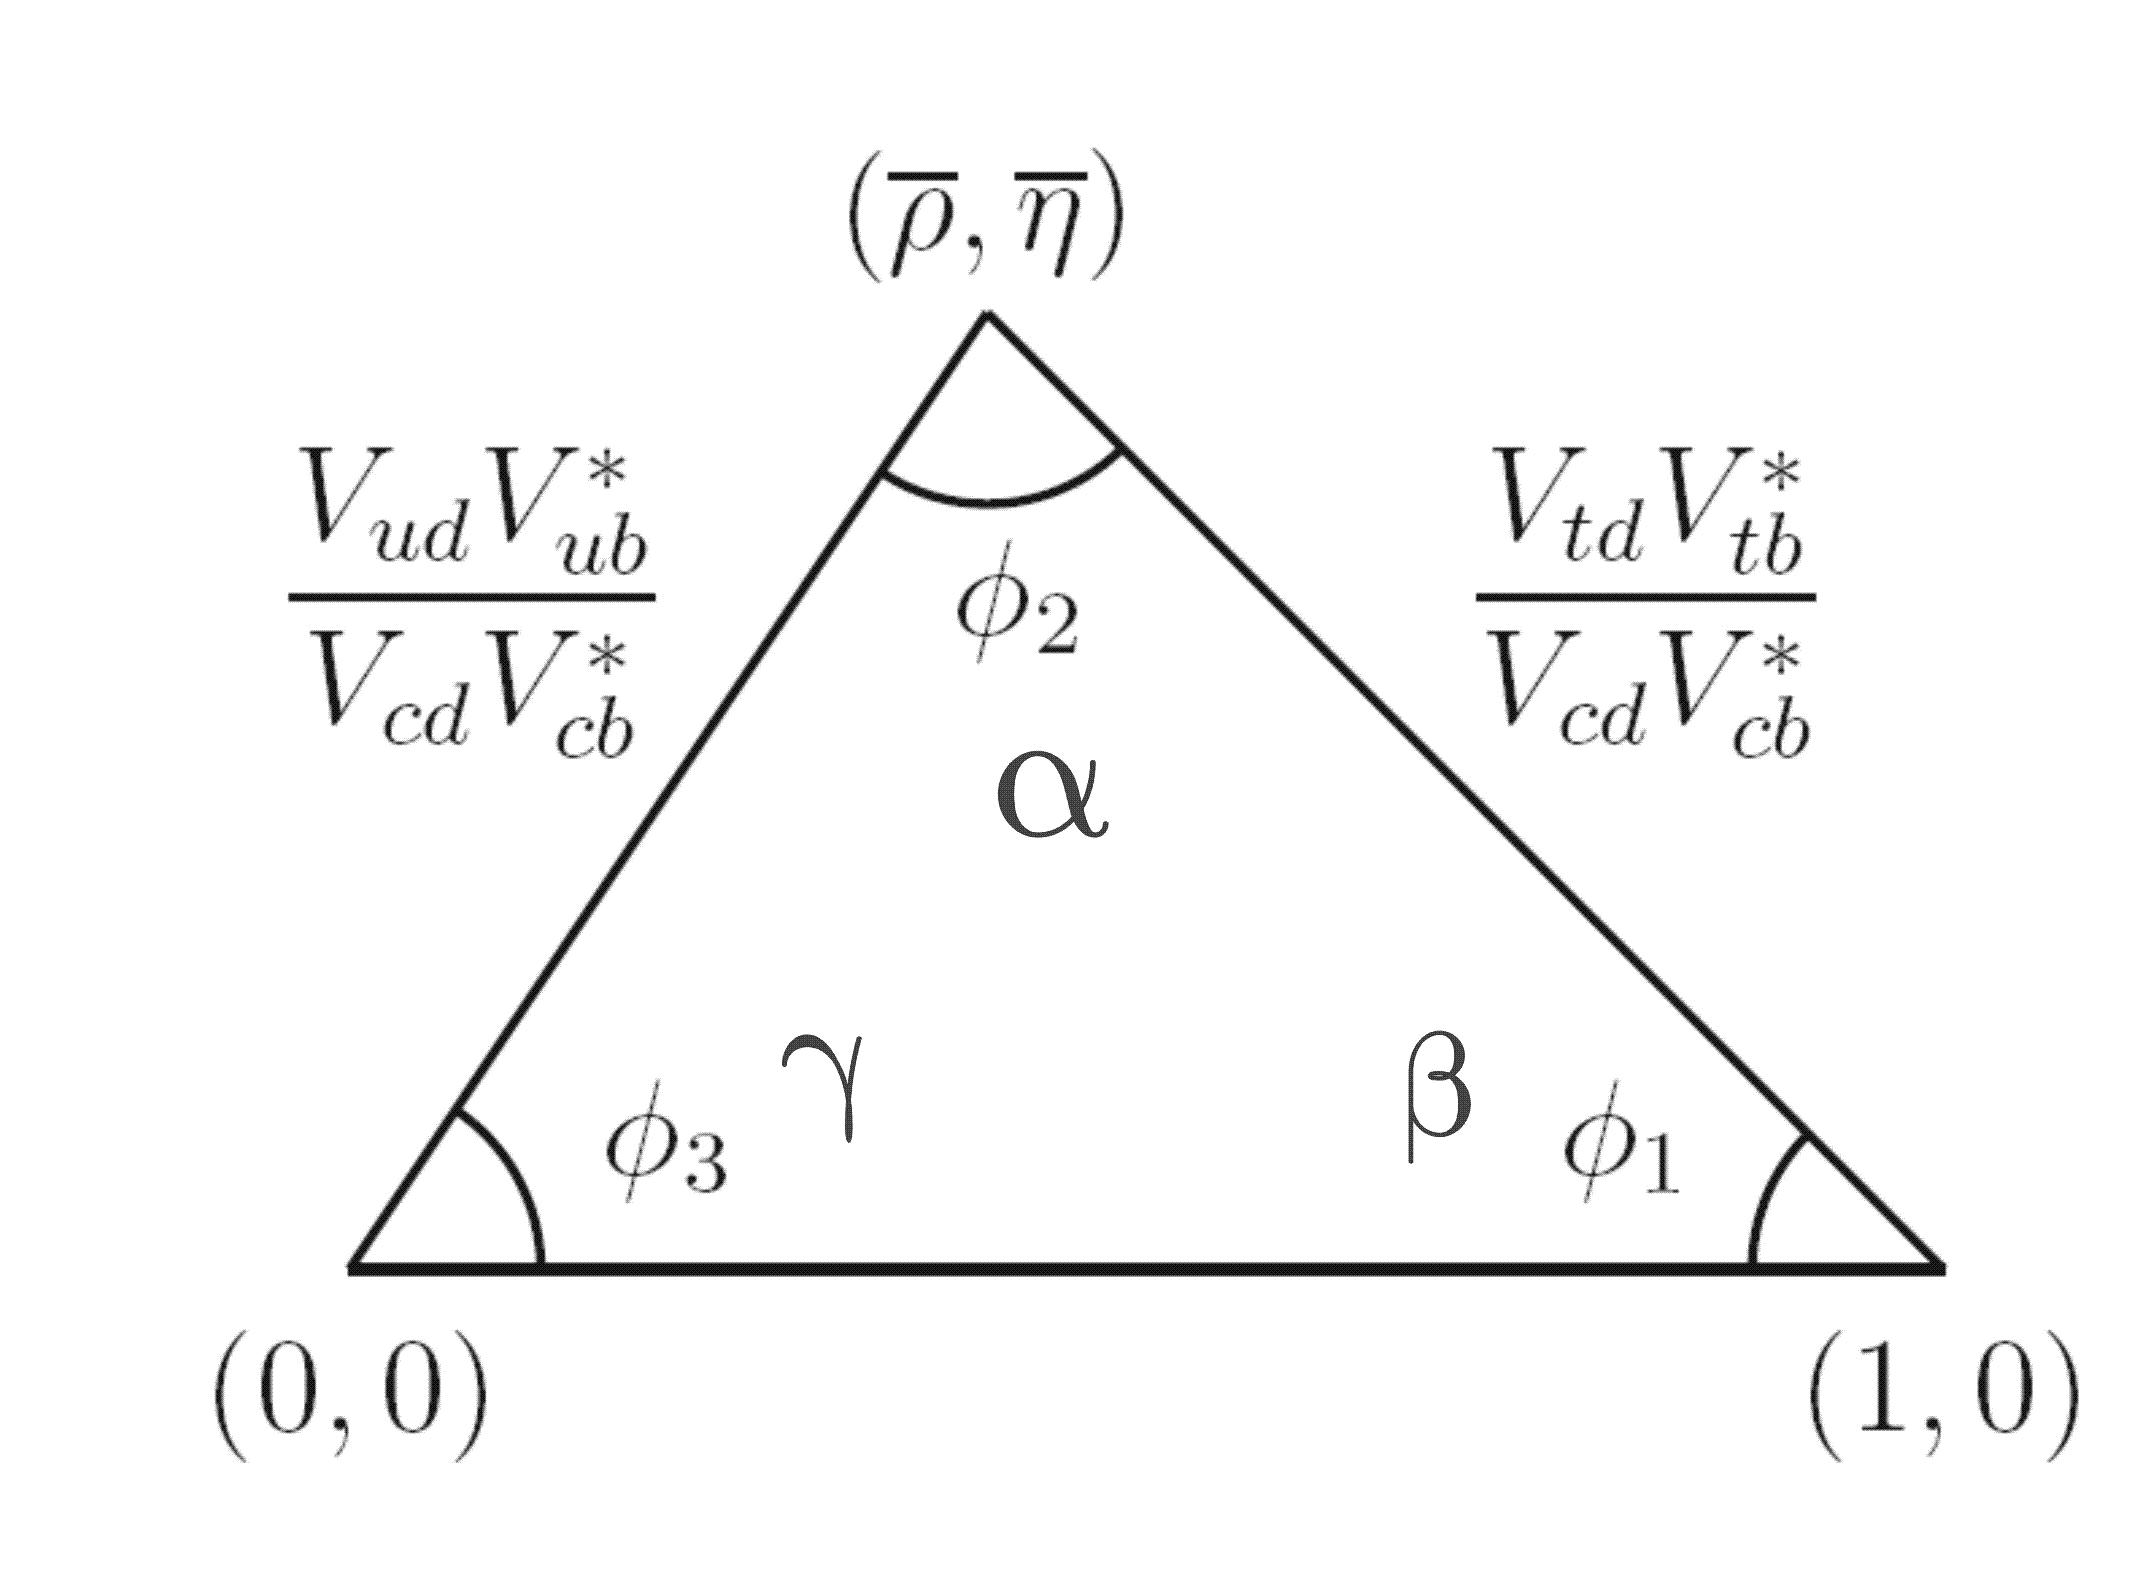
\includegraphics[width=0.8\textwidth]{Introduction/figs/Unitarity_triangle.png}
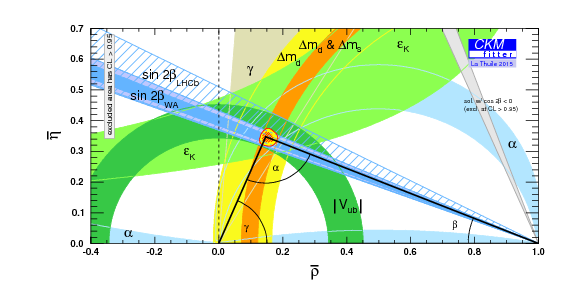
\includegraphics[width=0.8\textwidth]{Introduction/figs/Unitarity_triangle_HFAG.png}
\caption{(left) A representation of the unitarity triangle and its parameters.
(right) A summary of the most up to date measurements of the unitarity triangle parameters \cite{}.}
\end{figure}
 
 
 
 
\section{The puzzles in the SM}
\label{SMproblems}
Despite the confirmation of many predictions of the SM, this theory has several limitations and is unable to account for some observational facts.

\begin{itemize}
\item \emph{Dark matter}: From experimental evidence the content of visible matter in the universe is not enough
to account the observed rotation of galaxies \cite{Zwicky:1933gu} in the context of general relativity. 
Furthermore, studies of the fluctuations of the cosmic microwave background indicate the existence of
cold dark matter\cite{Dunkley:2008ie}, formed of particles which do not interact through the SM forces and
for which there is no SM candidate.

\item \emph{Matter-antimatter asymmetry}: We observe a large asymmetry between the quantity of matter and antimatter
in the Universe. Assuming that both were equally created in the initial state of the Universe, a condition such
as the violation of the CP symmetry is necessary to account for such observed differences. However the magnitude of
CP violation predicted by the SM is not enough to explain them \cite{Gavela:1993ts}.

\item \emph{Gravity}: There is not yet a consistent procedure to introduce gravity in the SM.

\item \emph{Neutrino oscillation}: By now, many measurements regarding solar and atmospheric neutrinos as wells as
neutrinos from nuclear reactor established that neutrinos can change flavour while propagating in space.
This is not predicted in the SM, in fact in the SM neutrinos are massless while an oscillation requires a non
zero mass \cite{Maltoni:2011zz}.

\item \emph{The mass hierarchy problem}: The mass of a scalar (spin 0 particle), such as the Higgs boson,
suffers from quantum corrections of its mass due to the physics above a certain scale
$\Lambda$, $m^2_{HSM} (phys) \sim m^2_{HSM} +  \frac{c}{16\pi}\Lambda^2$. Using the recently measured value
for the Higgs mass $\sim 126 ~\mbox{GeV/c}^2$\cite{Filippis:2013ana}, $\Lambda$ should be $\sim TeV$ in order
to avoid a fine tuning of the bare mass term.

\end{itemize}

\subsection{The flavour problem}

The SM has been very successful in describing the observed particles and their interactions so far. However, because
of its many puzzles, described in \ref{SMproblems}, it is believed only to be part of a more general theory or only
to be valid up to a certain energy scale. Many theoretical models expect New Physics (NP) to enter at the TeV scale.
For example, flavour conservation does not have a strong theoretical basis in the Standard Model and is mainly motivated
by experimental evidence.

So far we have talked about Flavour Changing Charged Currents (FCCC) that are mediated by the $W^\pm$ bosons. In the SM,
they are the only sources of flavour changing interaction and, in particular, of generation changing interactions,
where a quark or a lepton of a family transforms into one of an other family. There is no fundamental reason why there
cannot be Flavour Changing Neutral Currents (FCNCs). Yet, experimentally we see that FCNCs processes are highly suppressed.
The way in which the SM explains this is to forbid FCNC at tree level: since $Z$ and $\gamma$ interaction conserve flavour
the only other way to have FCNC is through particle loops. This makes this interactions very sensitive to new physics,
since its effects, which are expected to be small, are not disguised by dominating SM processes.

By now one of the possible explanations why we do not observe FCNC at tree level is the Minimal Flavour Violation (MFV)
hypothesis\cite{Isidori:2012ts}\cite{Buras:2003jf}, where FCNC are 'protected' by symmetry principles.


\section{Beyond the Standard Model}

From the last two sections it is evident that, despite the great success of the SM,
there is a need to explote new theories. Among the most promising approaches are those
invoking Super-Symmetry and extradimensions 

In Super-Symmetry new degrees of freedom are introduced to suppress the diverging term of the scalar mass. This represents
the main reasoning of Super-Symmetry, which assumes that for each fermion there is a corresponding boson. Since boson and
fermions contribute with opposite sign to the mass term they would cancel out if for each fermion we can add a boson term
\cite{Fayet:1976cr}.

The idea to introduce extra dimensions was triggered by the fact that normally gravity is not relevant
in particle physics at today's energy scales, which is at the EW scale ($\sim 100$ GeV), and this is why
it is neglected in the SM. However, adding extra dimensions to the normal 3 spatial dimensions,
one can restore some of the strength of gravity, yielding effects at the EW scale \cite{Randall:1999ee}.

In all these approaches severe contraints on masses and couplings must be imposed to maintain
compatibility with the SM at the electroweak scale.

\section{Flavour and BSM theories}

Since most of the BSM theories predict processes violating flavour, the observation or non-observation
of these processes can give important information about New Physics.

BSM theories can be classified according to the amount of flavour violation they introduce.
The first class of models to consider is the Minimal Flavour Violation (MFV).
These are models where the only sources of flavour violation in the SM and in BSM
are the different Yukawa couplings.
The MFV paradigm provides a way to resolve the tension between expectation, driven by naturalness arguments,
that NP should be at the \tev scale and limits on FCNC processes that point to much higher scales.
As hamiltonians for $\bquark\to\dquark$ and $\bquark\to\squark$ share the same structure,
ratios between these transitions provide powerful tests of MFV.
One particularly important example is the ratio of $\Bz$ and $\Bs$ dimuon decay rates \ref{}.

In the quest fot New Physics an important role is also played by simplified models
as a intermediate model building step. Instead of building models valid up to the GUT scale
one could consider simplified models including the SM and a new sector with a limited number
of parameters. Such models are easier to constrain but can nevertheless point in the right direction
to build a complete theory. The choice of the new sector to add can be driven by the need to
explain existing discrepancies between data and SM predictions or by theoretical prejudice.

Two models especially relevant for the discussion in this thesis are Z'-penguins and leptoquarks.

A Z'-penguin is a FCNC process involving a neutral field and as for the SM penguins it arises in
loops and modifications of the effective couplings arise in most SM extensions.
A survey of Z' models can be found in Ref. \cite{}.

Leptoquarks are bosonic particles that carry one quark and one lepton flavour quantum number.
They can be spin 1 but they ar more commonly assumed to be scalar particles.
A three level exchange of these particles induces processes such as $\bquark \to (\squark,\dquark)\ell\ell$
ans therefore we could observe an enhancement of their decay rates with respect to the SM.
Leptoquarks also provide a natural explanation for non-universal couplings to leptons,
introducing lepton flavour violation.


\section{Rare decays: a tool to search for new physics}

In the SM Flavour Changing Neutral Current processes, e.g. transitions from a
\bquark quark with charge of 1/3 to a \squark or \dquark with a charge of +2/3, 
are forbidden at tree level but can occur trough loops, box or penguin decays, see Fig.~\ref{fig:penguins}.
The branching fractions of this kind of decays is $\sim 10^{-6}$ or lower and therefore
they are called "rare decays". Additional NP contributions to the virtual loops
are not necessarily suppressed with respect to the SM component and this makes these decays
very sensitive to New Physics. Furthermore, this approach to New Physics searches is interesting as
New Physics could be at a high mass scale not accessible at colliders but its effect could be observed in loop effects.
Radiative and penguin decays are particularly interesting because they are theoretically
well understood which allows precise comparisons with measurements. Finally they provide
a great quantity of observables, not only decay rates, but also CP asymmetries and
angular observables can be affected by New Physics.

\begin{figure}[h!]
\centering
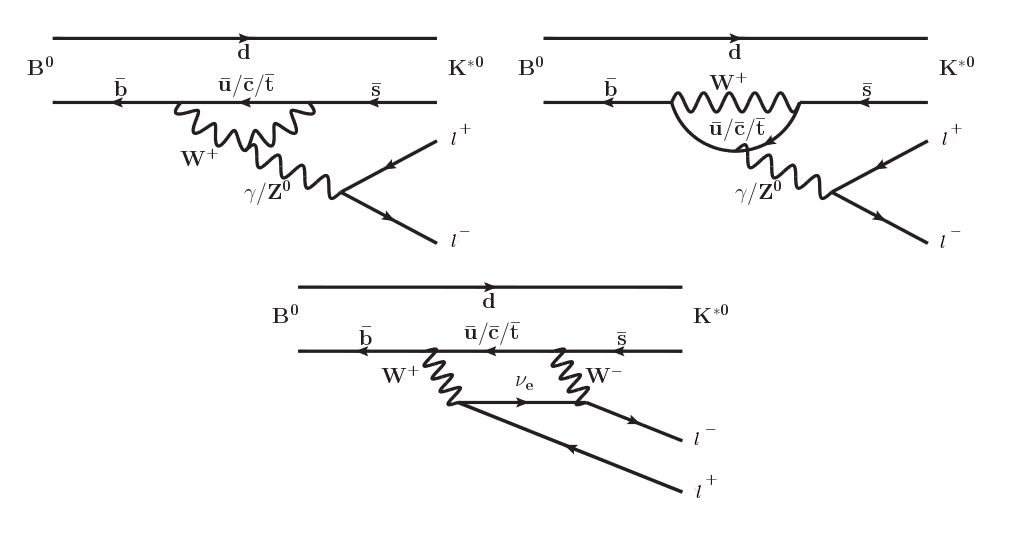
\includegraphics[width=0.8\textwidth]{Introduction/figs/penguins3.png}
\caption{Loop Feynmann diagrams for the rare $b \rightarrow s $ decay.}
\label{fig:penguins}
\end{figure}

\subsection{Theoretical framework: the effective Hamiltonian}
\label{sec:Effective_Hamiltonian}

Rare B decays are governed by an interplay between weak and strong interactions.
The QCD corrections that arise from hard gluon exchange bring large logarithms
of the form $\alpha_s^n(m_b)\log^m(m_b/M)$, where $M = m_t$ or $M = m_W$.
%A suitable framework to achieve the necessary resummation of these logarithms
%in an effective low-energy theory with five quarks.
The large masses of W, Z and top quark compared to that of the \bquark quark allow
the construction of an effective low-energy theory where the effective hamiltonian
can be written as:

\begin{equation}
\mathcal{H}_{eff} = \frac{4G_F}{\sqrt{2}} \sum C_i(\mu,M)\mathcal{O}_i(\mu)
\end{equation}

The method of the Operator Product Expansion (OPE) allows the separation
of the decay amplitudes into two parts: the long-distance contributions,
contained in the operator matrix elements, $\mathcal{O}_i$, and the short-distance physics described
by the so called Wilson Coefficients, $C_i$. $G_F$ denotes the Fermi coupling constant.

The weak coefficients at the weak scale can be obtained from matching amplitudes
of the full electroweak theory into $\mathcal{H}_{eff}$.
Then one can derive a renormalization group equation for the Wilson Coefficients

\begin{equation}
\mu \frac{\deriv}{\deriv \mu} C_i(\mu) = \gamma_{ij}C_j(\mu)
\end{equation}

where the matrix $\gamma$ is the anomalous dimensions matrix of the operators $\mathcal{O}_i$.
At leading order the solution is given by:

\begin{equation}
C_i(\mu) = \left[ \frac{\alpha_s(\mu_W)}{\alpha_s(\mu)}\right]^{\frac{\gamma^0_{ii}}{2\beta_0}} C_i(\mu_W) = \left[ \frac{1}{1 + \beta_0\frac{\alpha_s(\mu)}{4\pi}ln\frac{\mu_W^2}{\mu^2}} \right]^{\frac{\gamma^0_{ii}}{2\beta_0}} C_i(\mu_W)
\end{equation}

\subsection{Perturbative corrections}

The relevant efective Hamiltonian for $\bquark\to\squark\ell^+\ell^-$ transitions is

\begin{equation}
\mathcal{H}_{eff} = \frac{4G_F}{\sqrt{2}} \left[ V_{tb}V^*_{ts} \sum_{i=1}^{10} C_i \mathcal{O}_i \right]
% + V_{ub}V^*_{bs} \sum_{i=1}^{2} C_i ( \mathcal{O}_i - \mathcal{O}_i') \right]
\end{equation}

where the $V_{ub}$ and $V_{bs}$ are the factors of the CKM matrix.
The following local operators are particularly important for leptonic decays:

\begin{align}
& \mathcal{O}_7 = \frac{m_b}{e} \bar{s} \sigma^{\mu\nu}P_RbF_{\mu\nu}  			& \mathcal{O}_7' = \frac{m_b}{e} \bar{s} \sigma^{\mu\nu}P_LbF_{\mu\nu} \\
& \mathcal{O}_8 = g_s\frac{m_b}{e} \bar{s} \sigma^{\mu\nu}P_RT^abG^a_{\mu\nu}  	& \mathcal{O}_8' = g_s\frac{m_b}{e} \bar{s} \sigma^{\mu\nu}P_LT^abG^a_{\mu\nu} \\
& \mathcal{O}_9 = \bar{s} \gamma_{\mu}P_Lb\bar{\ell}\gamma^\mu\ell  			& \bar{s} \mathcal{O}_9' = \gamma_{\mu}P_Rb\bar{\ell}\gamma^\mu\ell \\
& \mathcal{O}_{10} = \bar{s} \gamma_{\mu}P_Lb\bar{\ell}\gamma^\mu\gamma_5\ell 	& \mathcal{O}_{10}' = \bar{s} \gamma_{\mu}P_Rb\bar{\ell}\gamma^\mu\gamma_5\ell \\
\end{align}


where $P_{L/R} = (1 \mp \gamma_5)/2$ denotes the left/right handed chiral projection,
$T^a$ are the QCD generators and $F_{\mu\nu}$ is the elecromagnetic field tensor.
The $\mathcal{O}'$ operators correspond to right-handed coupling obtained by swapping $P_R$ and $P_L$ in the equations.
The left-handedness of the weak interaction means that the $C'$ Wilson Coefficients are suppressed by $O(m_s / m_b)$ in the SM.

In the SM at $\mu_s = m_b$ the Wilson Coefficients have values:

%\begin{equation}
\begin{align}
& C_7^{SM} = -0.3, & C_9^{SM} = 4.2, & C_{10}^{SM} = -4.2. \\
\end{align}
%\end{equation}

New Physics contributions appear in the Wilson Coefficients as additive factors $C_i = C_i^{NP} + C_i^{SM}$

\subsection{Phenomenology of $\bquark\to\squark\ell\ell$ decays}
\label{sec:theo_qsq}

\begin{figure}[h!]
\centering
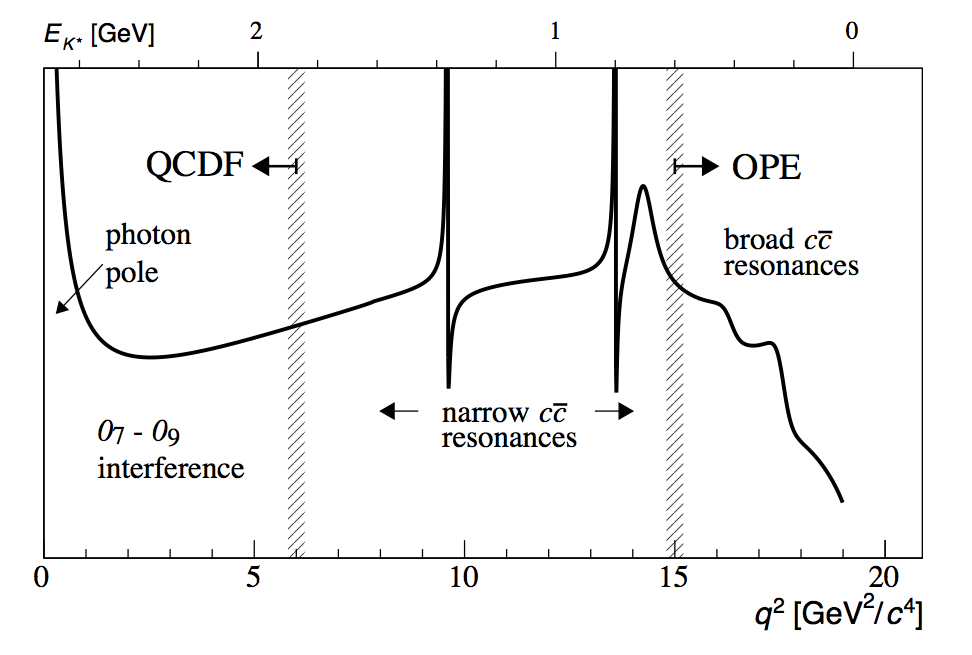
\includegraphics[width=0.8\textwidth]{fig/q2spectrum.png}
\caption{A typical $q^2$ spectrum of $\bquark\to\squark\ell\ell$ process characterised by the photon pole
at very low \qsq, charmonium resonances at central \qsq and broad resonances at high \qsq.}
\label{fig:q2spectrum}
\end{figure}

Semileptonic \bquark hadron decays are characterised by two kinematic regimes: at low \qsq, where the emitted hadron
is energetic ($E > \Lambda_{QCD}$ in the \bquark hadron rest frame), QCD factorisation applied; at high \qsq, the region
of low hadron recoil ($\qsq = O(m_b)$), an Operator Product Expansion (OPE) in $1/m_b$ applies.
In both regions decays can be predicted using the different methods and the biggest uncertainties come
from the limited knowledge of hadronic transition from factors.

As can be seen in Fig.~\ref{fig:q2spectrum} at very low \qsq the virtual photon contribution, associated with $C_7$, dominates.
In the region $1-6$ \gevgevcccc the interference between $C_7$ and $C_9$ becomes large, yielding sensitivity to NP in $C_9$.
The $6-15$ \gevgevcccc interval is dominated by charmonium resonances, \jpsi and \psitwos, though the tree level $b\to\cbar c s$ transition.
Although the decays can be experimentally vetoed in principle charmonia affect the entire \qsq space. 
Finally, at high \qsq borad charmonium resonances can contribute, like those observed by LHCb in $\decay{B^+}{K^+\mumu}$ decays \cite{}.

\subsection{Observables in $\bquark\to\squark\ell\ell$ decays}
\label{sec:observables}

Rare decays and especially semileptonic $\bquark\to\squark\ell\ell$ processes offer a pletora
of observables which can be used to search for New Physics.
The most direct effects appear in decay rates that can be enhanced by NP but the precision on
these measurements is often by uncertainty of form factor calculations or charm loops.
Therefore it is important also to look for different observable.
One important class of observables are angular quantities that can carry information about NP,
often complementary to branching ratio measurements. The most basic of these observable are
forward-backward asymmetries that characterise the angular distribution of final particles.
For the \Bz\to\Kstar\mumu decay combination of observables have been proposed that are 
independent of form factor uncertainties in the fits order \cite{}.
One more way to build stable observable is t/o construct ratios between similar
decays in which, for example, uncertainties due to the hadronisation process cancel out.
These observables include the $R_H$ ratios, between \Bz decay into electrons and muons,
that are described in detail in Sec.~\ref{sec:RKst_theory}.


\section{Experimental status}

In order to set the background for the searches included in this thesis, in this section a review of recent
or important results of NP searches involving rare decays or lepton flavour violation.
Among these, results recently obtained by the \lhcb experiment show a series of anomalies
with respect to the SM that have the potential to yield to NP scenarios.


\subsection{Dimuon decays of \bquark hadrons}

Decays of $B$ mesons into two muons have been recently studies at the \lhcb and \cms experiments.
These are two-body decays where the two muons are back to back in the hadron rest frame.
The simple signatures of these decays makes them easy to study and the fact that they
are unaffected by hadronic physics in the final state makes predictions very clean and precise.
Therefore these are essential tests for the SM.
The $\decay{\Bz}{\mumu}$ and $\decay{\Bz}{\mumu}$ decays are exceedingly rare in the SM.
First of all they can only happen in loops and furthermore they are CKM-suppressed.
In addition to that the decay of a pseudo-scalar $B$ meson into two muons has a significant helicity suppression.
The latest SM predictions for these decay rates are \cite{}:
%
\begin{align}
\mathcal{B}(\decay{\Bs}{\mumu}) = (3.65 \pm 0.23) \times 10^{-9} \text{ and } \\
\mathcal{B}(\decay{\Bz}{\mumu}) = (1.06 \pm 0.09) \times 10^{-10}.
\end{align}
%
The uncertainties on these values mainly comes from the knowledge of the decay constants and CKM-elements.
BSM models, for example models with extended Higgs sectors can produce significant enhancement to
these decays. Furthermore the measurement of their ratio is a stringent test of the MFV hypothesis.
A combination of the \lhcb and \cms results resulted in the measured values \cite{}:
%
\begin{align}
\mathcal{B}(\decay{\Bs}{\mumu}) = (2.8^{+0.7}_{-0.6}) \times 10^{-9} \text{ and } \\
\mathcal{B}(\decay{\Bz}{\mumu}) = (3.9^{+1.6}_{-1.4}) \times 10^{-10}.
\end{align}
%
Both decays where unobserved and now the $\Bs$ decay was observed with a significance of $6\sigma$
and evidence for the $\Bz$ decay was found with a $3\sigma$ significance.
These are compatible with SM predictions within $2\sigma$ and put strong contraints to
the available parameter-space for BSM theories.

\subsection{Semileptonic $\bquark\to\squark\ell\ell$ decays of \bquark hadrons}

Many branching ratios of semileptonic $B$ meson decays where recently measured at the \lhcb experiment,
including $\decay{B}{K\mumu}$, $\decay{B}{K*\mumu}$ and $\decay{\Bs}{\phi\mumu}$ \cite{}.
Baryon decays where also studied at \lhcb: including the branching ratio of
the rare $\decay{\Lambda_b}{\Lz\mumu}$ decay \cite{}, which is described in this thesis.
For semileptonic decays, unlike for dilepton decays, SM predictions are affected by the
knowledge of hadronic form factors, {\em describing phsycis bla bla}. This typically yields
to uncertainties of $\mathcal{O}(30\%)$.
As described in \ref{sec:observables} many observables can be affected by 


\subsection{Lepton Flavour Violation searches}

Several LFV searches are linked to rare decays as they involve small branching ratios
in the SM that can be enhances by NP. They are therefore a natural place to look for NP.
Lepton flavour conservation is well experimentally established but has no strong theoretical explanation
and in fact we already know that flavour is not conserved in neutrino oscillations.
In this section is reported a short review of Lepton Flavour Violation searches.
The best-studied decays violating lepton flavour are rare muon decays including $\mu^+\to e^+\gamma$
and $\mu^+\to e^+e^-e^+$. Since muons can be abundantly produced and the final states are simple,
these decays provide the best constraints to LFV. The present best-upper limits are $1.2 \times 10^{-11}$
for the radiative decay and $1.0 \times 10^{-12}$ for $\mu^+\to e^+e^-e^+$ obtained respectively by the
MEGA \cite{} and SINDRUM \cite{} experiments.

Several LFV searches have been recently been performed at the LHCb experiment including $B$ meson
decays such as $\Bz\to e\mu$ \cite{} and $\tau$ decays such as $\tau\to\mumu\mu$ \cite{}.
None of these searches has found evidence of NP so far and therefore they set limits, constraining
the parameter space available for NP models. Fig.~\ref{fig:LFV_decay} reports a summary of
the best limits on LFV searches.


\begin{figure}[h!]
\label{fig:LFV_decay}
\centering 
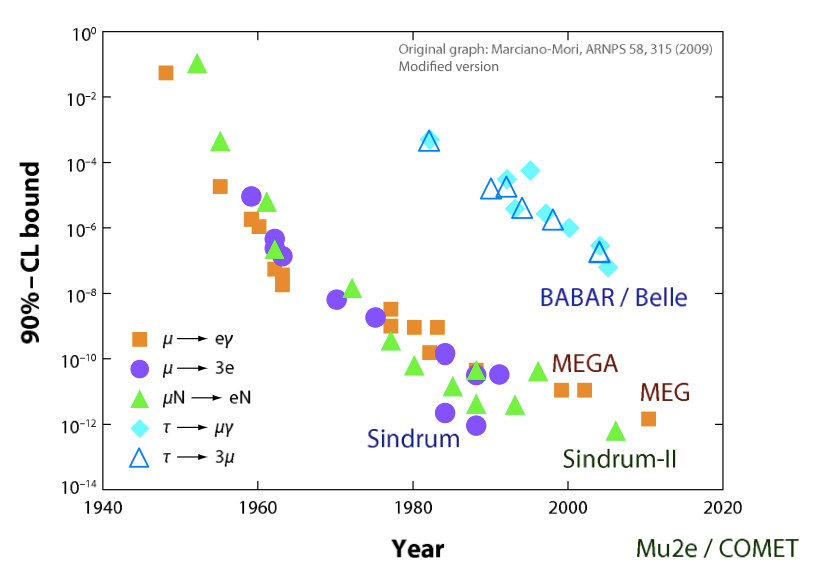
\includegraphics[width=0.8\textwidth]{Introduction/figs/LFV.png}
\caption{Summary of limits set in lepton flavour violation searches \cite{}.}
\end{figure}
 